\documentclass[aspectratio=169]{beamer}
\usepackage[utf8]{inputenc}
%\usepackage[authordate,backend=biber,natbib]{biblatex-chicago}
%\usepackage{booktabs}
%\addbibresource{growthreferences.bib}

%\usepackage{utopia} %font utopia imported

\usetheme{Madrid}
\usecolortheme{beaver}

%------------------------------------------------------------
%This block of code defines the information to appear in the
%Title page
\title[Bagwell and Staiger (1996)] %optional
{Reciprocal Trade Liberalization}

\subtitle{Kyle Bagwell and Robert Staiger, NBER Working Paper, 1996}

\author [Hauk] % (optional)
{William~R.~Hauk,~Jr.} %\inst{1} %\and J.~Doe\inst{2}} 

\institute[UofSC] % (optional)
{
  %\inst{1}%
  Darla Moore School of Business\\
  University of South Carolina
  %\and
  %\inst{2}%
  %Faculty of Chemistry\\
  %Very Famous University
}

\date[ECON 860, Fall 2021] % (optional)
{ECON 860 -- International Trade Theory\\Fall 2021}

\logo{
\includegraphics[height=1cm]{UofSC_Monogram_Stack_CMYK_G.jpg}}

%End of title page configuration block

%---------------------------------------------------------

\AtBeginSection[]
{
  \begin{frame}
    \frametitle{Table of Contents}
    \tableofcontents[currentsection]
  \end{frame}
}

%------------------------------------------------------------

\begin{document}

%The next statement creates the title page.
\frame{\titlepage}

%-------------------------------------------------------------

\section{Introduction}

%-------------------------------------------------------------

\begin{frame}{Multilateralism in Trade}

\begin{itemize}
    \item<1-> Two major principles of international trade have dominated the post-World War II trading order – reciprocity and nondiscrimination – and they are enshrined the in the charters of the WTO and its predecessor, the GATT.
    \item<2-> \textbf{Reciprocity --} the balance of concessions that governments seek to obtain through negotiation (i.e. I lower my tariffs if you lower yours)
    \item<3-> \textbf{Nondiscrimination --} the requirement that each country adopt a uniform trade policy across trading partners (the ``Most-Favored Nation” principle, no country-specific tariffs)
\end{itemize}
    
\end{frame}

%-------------------------------------------------------------

\begin{frame}{Multilateralism Puzzle}

\begin{itemize}
    \item<1-> Trade protection is usually harmful to the country engaging in it – so why to we need reciprocal multilateral agreements?
    \item<2-> Mercantilist perspective – exports good, imports bad – makes some sense from a political perspective, even if it isn’t good economics.
    \item<3-> A more economically-based argument is that trade agreements can help to resolve a prisoner’s dilemma if there are terms-of-trade effects between large countries, but terms-of-trade arguments give countries an incentive to tax exports, which we rarely see.
\end{itemize}
    
\end{frame}

%-------------------------------------------------------------

\begin{frame}{Paper's Motivations}

\begin{itemize}
    \item<1-> Purpose of paper is develop a formal model in which both motivations can be assessed.
    \item<2-> First model is a two-country general equilibrium model that allows for a wide range of possible government motivations.  Government preferences represented as a general function of local prices and world prices.
    \item<3-> In the second model, preferences are more explicit, and government places a heavier weight on producer surplus than consumer surplus (which, they note, could be an implication of the Grossman and Helpman (1994) model).
\end{itemize}
    
\end{frame}

%-------------------------------------------------------------

\begin{frame}{Main Conclusions}

\begin{itemize}
    \item<1-> ``While political concerns can influence a government’s goals, however, they play no role in explaining why reciprocal trade agreements (as opposed to unilateral policies) can help reach those goals… The central purpose of a reciprocal trade agreement is to eliminate the terms-of-trade driven trade restrictions that arise in the absence of such an agreement."
    \item<2-> Governments tend to oversupply policies directed towards import protection and undersupply policies directed towards export promotion – even though both would benefit producers.  (Import protection has positive terms-of-trade effect, export promotion has negative terms-of-trade effect).
\end{itemize}
    
\end{frame}

%-------------------------------------------------------------

\begin{frame}{Reciprocity and Nondiscrimination}

\begin{itemize}
    \item<1-> Secondary purpose of the paper is to offer an economic interpretation of the principles of reciprocity and nondiscrimination at the heart of the GATT and WTO.
    \item<2-> More efficient outcomes are attainable under reciprocity – the terms-of-trade implications of each country’s own liberalization are neutralized.
    \item<3-> Therefore, a major obstacle preventing unilateral trade liberalization is removed.
    \item<4-> Nondiscrimination in trade helps to prevent beggar-thy-neighbor policies.
\end{itemize}
    
\end{frame}

%-------------------------------------------------------------

\section{Reciprocal Trade Agreements in a Two-Country General-Equilibrium Framework}

%-------------------------------------------------------------

\begin{frame}{Reciprocal Trade Agreements in a Two-Country General-Equilibrium Framework}

\begin{itemize}
    \item<1-> Two countries, home and foreign, trade two goods, $ x $ and $ y $, produced under conditions of increasing opportunity costs.  Assume perfect competition.
    \item<2-> Let $ x $ by the natural import good of the home country and $ y $ for the foreign country.  Define  $ p  = \frac{p_{x}}{p_{y}} $ be the local relative price for consumers in the home country, and $ p^{*} = \frac{p^{*}_{x}}{p^{*}_{y}} $ be the relative price for consumers in the foreign country.
    \item<3-> Let $ t $ represent the home ad-valorem tariff on the import good (which we assume is non-prohibitive).  Let $ \tau =  \left( 1 + t \right) $ so that $ p = \tau p^{w} $ and similarly $ p^{*} = \frac{p^{w}}{\tau^{*}} $. 
\end{itemize}
    
\end{frame}

%-------------------------------------------------------------

\begin{frame}{World Prices and Terms of Trade}

\begin{itemize}
    \item<1-> $ p^{w} = \frac{p_{x}^{*}}{p_{y}} $ is the ``world" relative price without taxes.
    \item<2-> The foreign terms of trade is thus $ p^{w} $ and the home terms of trade is $ \frac{1}{p^{w}} $. 
\end{itemize}
    
\end{frame}

%-------------------------------------------------------------

\begin{frame}{Production, Imports, and Exports}

\begin{itemize}
    \item<1-> Production in each country is determined by finding the point on the production possibilities frontier where the marginal rate of transformation between $ x $ and $ y $ is equal to the local relative price, so $ Q_{i} = Q_{i}\left( p \right) $ and $ Q_{i}^{*} = Q_{i}^{*}\left( p^{*} \right) $ for both goodes $ x $ and $ y $.
    \item<2-> Consumption is also determined by local and world relative prices, the latter mattering due to the lump-sum distribution of tariff revenue to households, so that $ C_{i} = C_{i}\left( p, p^{w} \right) $ for both goods and both countries.
    \item<3-> Home country imports of $ x $ are given by $ M_{x}\left( p\left( \tau, p^{w} \right), p^{w} \right) $ and home country exports of $ y $ are given by $ E_{y}\left( p\left( \tau, p^{w} \right), p^{w} \right) $ and vice cersa for foreign country exports of $ x $ and imports of $ y $.
\end{itemize}
    
\end{frame}

%-------------------------------------------------------------

\begin{frame}{World Prices}

\begin{itemize}
    \item<1-> Balanced trade occurs at the point where:
    \begin{equation*}
        p^{w} M_{x}\left( p\left( \tau, p^{w} \right), p^{w} \right) = E_{y}\left( p\left( \tau, p^{w} \right), p^{w} \right)
    \end{equation*}
    \item<2-> And the equilibrium world price $ \tilde{p}^{w} $ is determined by the point where:
    \begin{equation*}
        E_{y}\left( p\left( \tau, \tilde{p}^{w} \right), \tilde{p}^{w} \right) = M_{y}^{*}\left( p^{*}\left( \tau^{*}, \tilde{p}^{w} \right), \tilde{p}^{w} \right)
    \end{equation*}
\end{itemize}
    
\end{frame}

%-------------------------------------------------------------

\begin{frame}{Government Preferences}

\begin{itemize}
    \item<1-> Government objective functions are deliberately flexibly specified as:
    \begin{equation*}
        W\left( p\left( \tau, \tilde{p}^{w}\left( \tau, \tau^{*} \right) \right), \tilde{p}^{w}\left( \tau, \tau^{*} \right) \right)
    \end{equation*}
    and similarly for the foreign government.
    \item<2-> These objective functions could include national income maximization goals, but they could also include things like income distribution within the country or political economy concerns that are affected by relative prices within the countries.
    \item<3-> The main structure placed on these functions is that a positive terms of trade change will, holding local prices constant, have a positive change on government welfare, so that:
    \begin{equation*}
        \frac{\partial W\left( p, p^{w} \right)}{\partial p^{w}} < 0 \text{ and } \frac{\partial W^{*}\left( p^{*}, p^{w} \right)}{\partial p^{w}} > 0
    \end{equation*}
\end{itemize}
    
\end{frame}

%-------------------------------------------------------------

\subsection{A Role for Reciprocal Trade Agreements}

%-------------------------------------------------------------

\begin{frame}{A Role for Reciprocal Trade Agreements}

\begin{itemize}
    \item<1-> We start by assuming that each government sets its trade policy unilaterally, taking the other government’s policy as given.  The reaction function for the home country is defined implicitly as $ \frac{\partial W}{\partial p} \frac{\partial p}{\partial \tau} + \frac{\partial W}{\partial p^{w}} \frac{\partial p^{w}}{\partial \tau} = 0 $ and for the foreign country as $ \frac{\partial W^{*}}{\partial p^{*}} \frac{\partial p^{*}}{\partial \tau^{*}} + \frac{\partial W^{*}}{\partial p^{w}} \frac{\partial p^{w}}{\partial \tau^{*}} = 0 $.
    \item<2-> We assume that $ \frac{\partial p}{\partial \tau} > 0 $, $ \frac{\partial p^{*}}{\partial \tau^{*}} < 0 $, $ \frac{\partial p^{w}}{\partial \tau} < 0 $, and $ \frac{\partial p^{w}}{\partial \tau^{*}} > 0 $.
    \item<3-> If we redefine $ \lambda = \frac{\partial p^{w}}{\partial \tau} / \frac{\partial p}{\partial \tau} < 0 $ and $ \lambda^{*} = \frac{\partial p^{w}}{\partial \tau^{*}} / \frac{\partial p}{\partial \tau^{*}} > 0 $, this can be rewritten as:
    \begin{align}
        \frac{\partial W}{\partial p} + \lambda \frac{\partial W}{\partial p^{w}} &= 0 \label{eq:homefoc} \\
        -\frac{\partial W^{*}}{\partial p^{*}} - \lambda^{*} \frac{\partial W^{*}}{\partial p^{w}} &= 0 \label{eq:foreignfoc}
    \end{align}
\end{itemize}
    
\end{frame}

%-------------------------------------------------------------

\begin{frame}{Nash Equilibrium}

\begin{itemize}
    \item<1-> Two forces combine to determine trade policy when government’s set tariffs non-cooperatively – the impact of tariffs on local prices and the impact of tariffs on the terms of trade.
    \item<2-> Because of the terms of trade effects in (\ref{eq:homefoc}) and (\ref{eq:foreignfoc}), each government will not face the full costs of their tariff policies when setting them non-cooperatively.  Nash equilibrium will not be a Pareto-efficient policy.
    \item<3-> The purpose of a reciprocal trade agreement (RTA), then, is to internalize these ``externalities" through mutual reductions in trade barriers.
\end{itemize}
    
\end{frame}

%-------------------------------------------------------------

\begin{frame}{Efficiency and Proposition \#1}

An efficient RTA will move governments to the Pareto efficiency locus, defined as:
\begin{equation}
    \left[ \frac{d \tau}{d \tau^{*}} \right]_{dW = 0} = \left[ \frac{d \tau}{d \tau^{*}} \right]_{dW^{*} = 0}
    \label{eq:efficientlocus}
\end{equation}
\begin{theorem}{Proposition \#1}
    Nash Equilibrium Tariffs are inefficient.
\end{theorem}
Proposition \#1 therefore implies that Pareto Improvements could be obtained relative to a Nash Equilibrium via a reciprocal trade agreement. 

\end{frame}

%-------------------------------------------------------------

\begin{frame}{Proof of Proposition \#1}

\begin{proof}
    Note that:
    \begin{align}
        \left[ \frac{d \tau}{d \tau^{*}} \right]_{dW = 0} &= -\frac{\partial p^{w} / \partial \tau^{*}}{d p / d \tau}\left[ \frac{\tau \frac{\partial W}{\partial p} + \frac{\partial W}{\partial p^{w}}}{\frac{\partial W}{\partial p} + \lambda \frac{\partial W}{\partial p^{w}}} \right] \label{eq:dtaudtau*home} \\
        \left[ \frac{d \tau}{d \tau^{*}} \right]_{dW^{*} = 0} &= -\frac{d p^{*} / d \tau^{*}}{\partial p^{w} / \partial \tau}\left[ \frac{\frac{\partial W^{*}}{\partial p^{*}} + \lambda \frac{\partial W^{*}}{\partial p^{w}}}{\frac{\partial W^{*}}{\partial p^{*}} / \tau^{*} + \frac{\partial W^{*}}{\partial p^{w}}}{} \right] \label{eq:dtaudtau*foreign}
    \end{align}
    At the pair of Nash Equilibrium tariffs, $ \left( \tau^{N}, \tau^{* N} \right) $, $ \left[ \frac{d \tau}{d \tau^{*}} \right]_{dW = 0} = \infty $, and $ \left[ \frac{d \tau}{d \tau^{*}} \right]_{dW^{*} = 0} = 0 $, so clearly these two derivatives are not equal in the Nash Equilibrium.  By the definition offered above, then, they are not efficient.  \textbf{Q.E.D.}
\end{proof}
    
\end{frame}

%-------------------------------------------------------------

\begin{frame}{Figure 1}

\begin{figure}
    \centering
    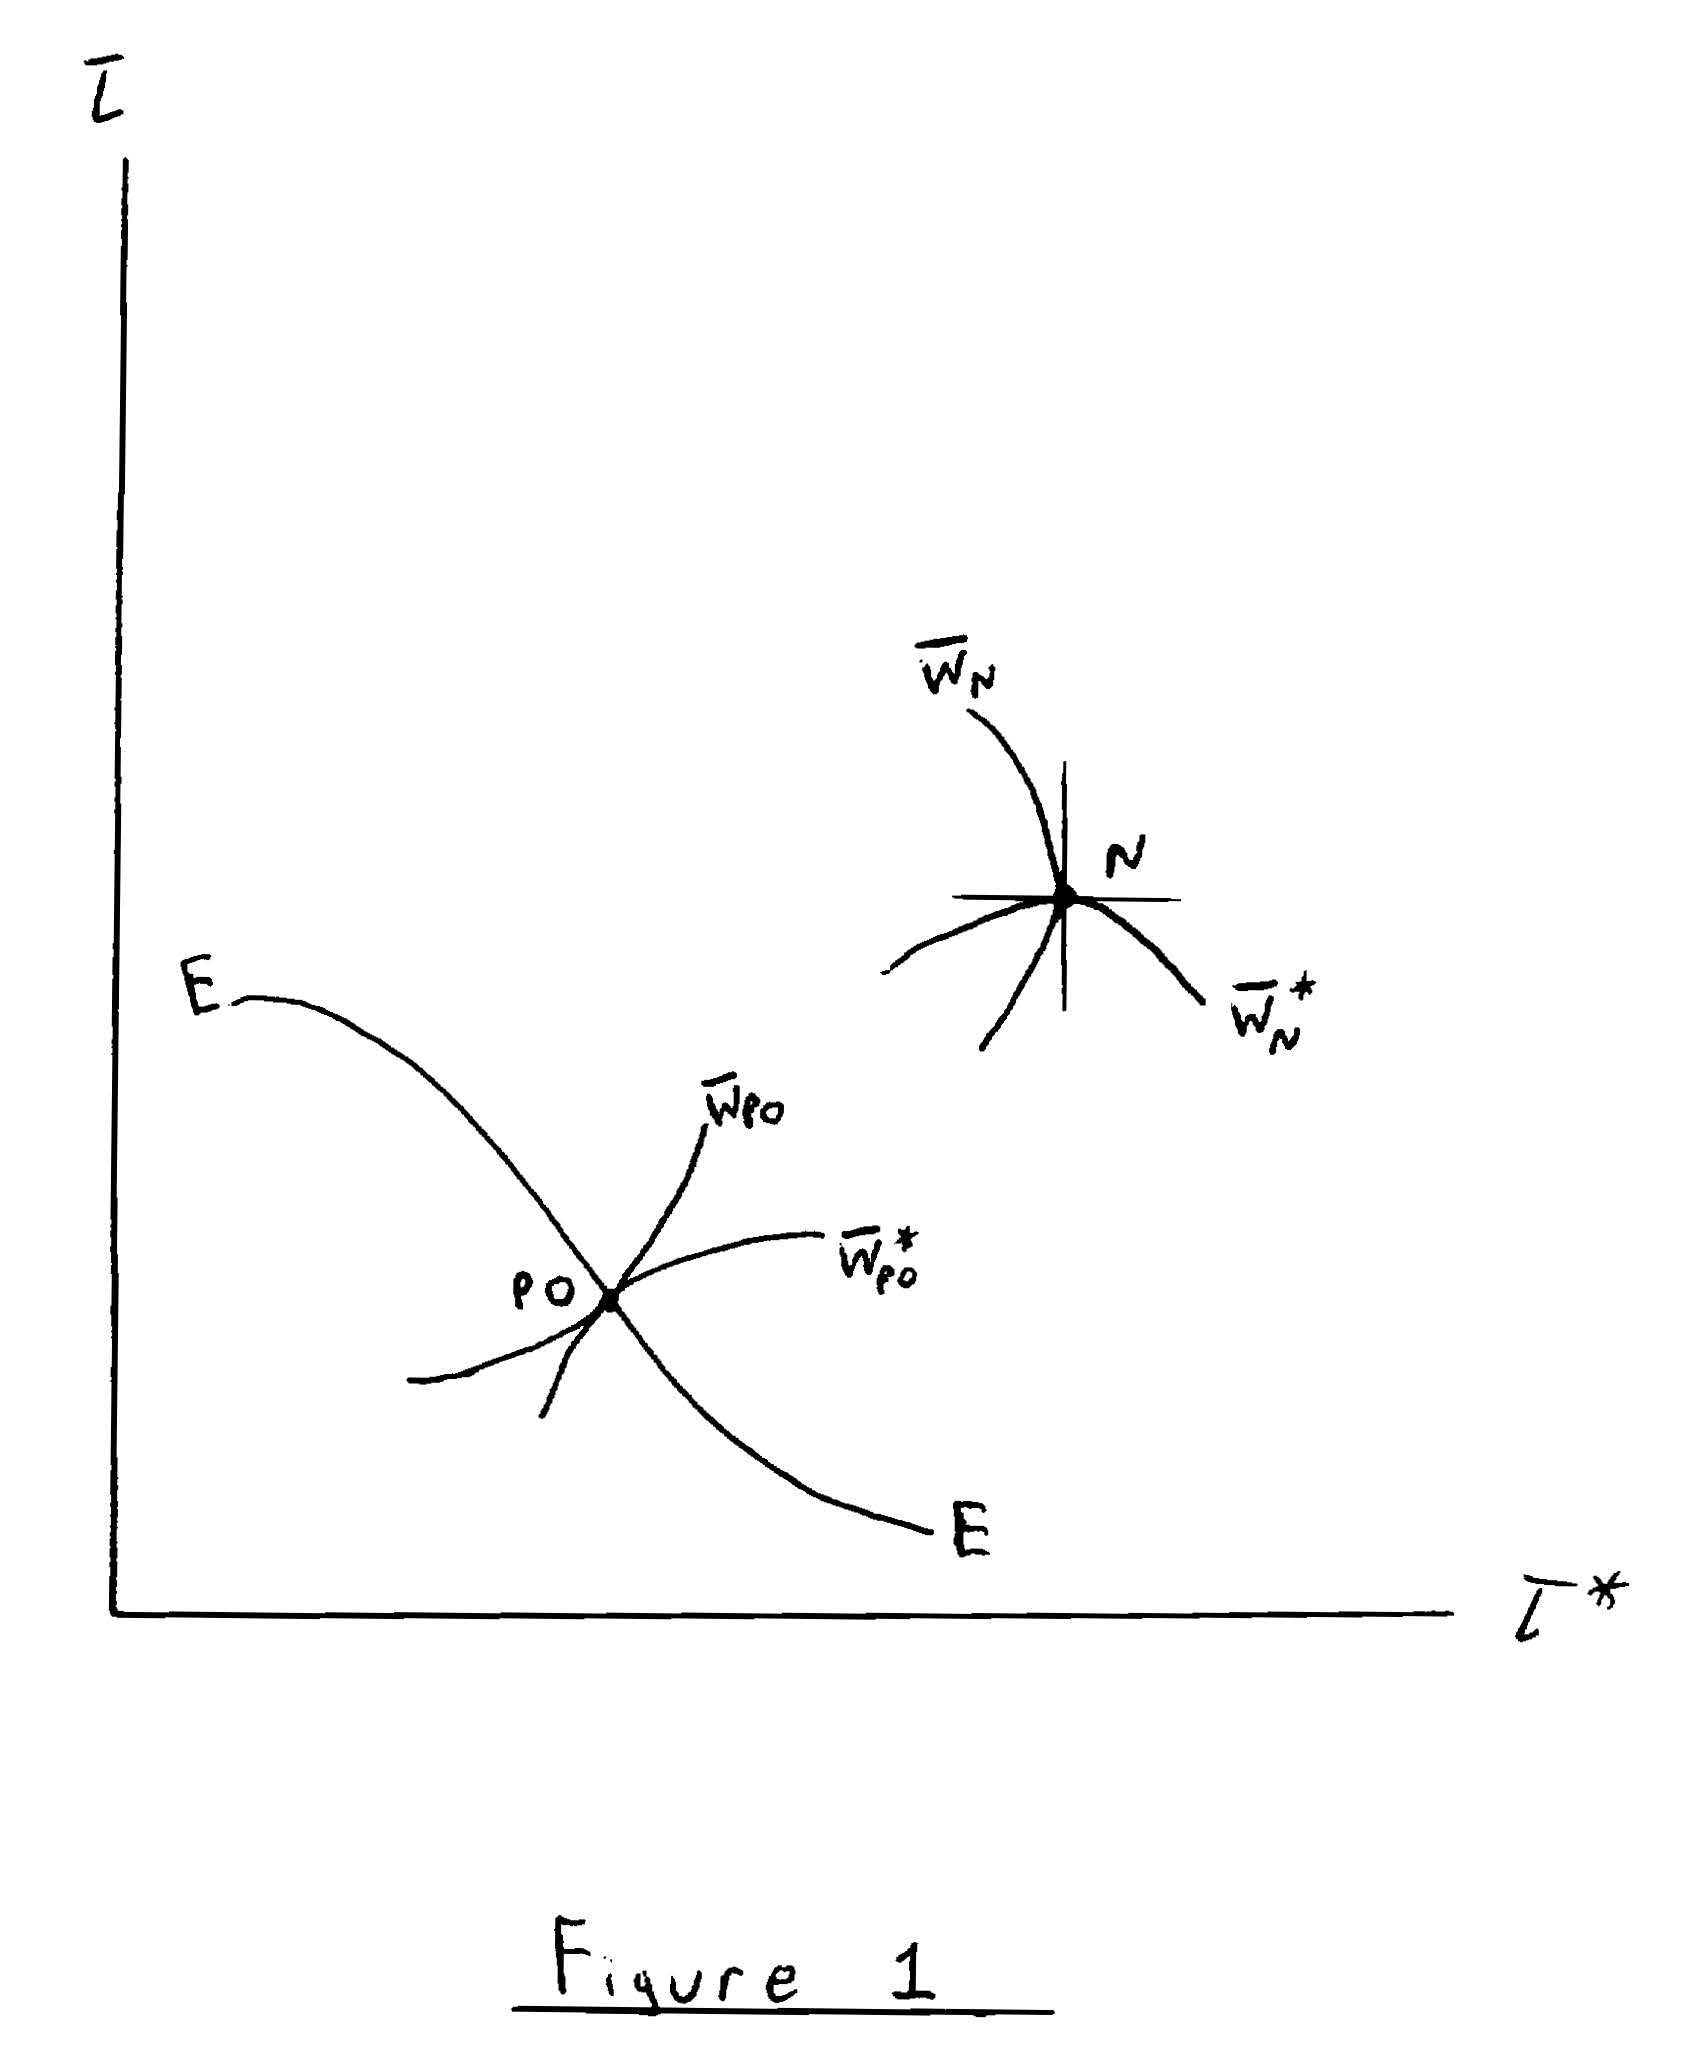
\includegraphics[scale=0.4]{BagwellStaigerFig1.jpg}
    \label{fig:Fig1}
\end{figure}
    
\end{frame}

%-------------------------------------------------------------

\begin{frame}{Proposition \#2}

\begin{theorem}{Proposition \#2}
    Starting from a Nash Equilibrium, any reciprocal trade agreement that is mutually beneficial must entail reciprocal trade liberalization.
\end{theorem}
The idea is that a necessary condition for any tariff pair $ \left( \tau^{0}, \tau^{0 *} \right) $ to yield welfare improvements for both the foreign and domestic governments relative to Nash Equilibrium tariffs, it must be the case that $ \tau^{0} < \tau^{N} $ and $ \tau^{0*} < \tau^{N*} $
\begin{proof}
    To establish this, show that if $ \tau^{0} > \tau^{N} $, then the foreign government must lose.  Recall that equations (\ref{eq:homefoc}) and (\ref{eq:foreignfoc}) implicitly define the home and foreign reaction curves from changes in tariffs.  Therefore the change in foreign government welfare from a change in $ \tau $  by the home country is:
    \begin{equation}
        \frac{d W^{*}}{d \tau} = \left[ 1 - \frac{\lambda^{*}}{\tau^{*} R\left( \tau \right)} \right] \frac{\partial W^{*}}{\partial p^{w}} \frac{\partial p^{w}}{\partial \tau} < 0
        \label{eq:dW*dtau}
    \end{equation}
\end{proof}

\end{frame}

%-------------------------------------------------------------

\begin{frame}{Proposition \#2 Proof, continued}

\begin{proof}
    The term in brackets from equation (\ref{eq:dW*dtau}) is positive so long as the tariff ``pass-through" on world prices isn’t 100\%.  $ \frac{\partial W^{*}}{\partial p^{w}} > 0 $ because $ p^{w} $ is the relative price of the foreign country’s export good, and $ \frac{\partial p^{w}}{\partial \tau} < 0 $ due to the terms of trade effect. \\
    In words, if the home government raises its tariff level beyond the Nash Equilibrium, the foreign government would either have the suffer the terms-of-trade loss, which would lower its welfare, or raise its own tariff, which would also lower its welfare. \\
    Analogous arguments would establish that the home government would be hurt by an increase in the foreign tariff above Nash Equilibrium levels. \textbf{Q.E.D.}
\end{proof}
    
\end{frame}

%-------------------------------------------------------------

\begin{frame}{Politically Optimal Tariffs}

Define politically optimal tariffs $ \left( \tau^{PO}, \tau^{PO*} \right) $ as the outcome of a reciprocal trade agreement that eliminates the terms of trade motivation from each government’s trade policy decisions and implements tariffs that jointly satisfy:
\begin{align}
    \frac{\partial W}{\partial p} &= 0 \label{eq:dWdp} \\
    \frac{\partial W^{*}}{\partial p^{*}} &= 0 \label{eq:dW*dp*}
\end{align}

\begin{theorem}{Proposition \#3}
    Politically optimal tariffs are efficient.
\end{theorem}
    
\end{frame}

%-------------------------------------------------------------

\begin{frame}{Proof of Proposition \#3}

\begin{proof}
    Combining equations (\ref{eq:dWdp}) and (\ref{eq:dW*dp*}) with equations (\ref{eq:dtaudtau*home}) and (\ref{eq:dtaudtau*foreign}) we know that:
    \begin{equation*}
        \left[ \frac{\partial \tau}{\partial \tau^{*}} \right]_{dW = 0} = -\frac{\partial p^{w} / \partial \tau^{*}}{\partial p^{w} / \partial \tau} = \left[ \frac{\partial \tau}{\partial \tau^{*}} \right]_{dW^{*} = 0}
    \end{equation*}
    which means that these tariffs are efficient. \textbf{Q.E.D.}
\end{proof}
    
\end{frame}

%-------------------------------------------------------------

\begin{frame}{Sufficiency and Necessity}

\begin{itemize}
    \item<1-> Proposition \#3 tells us that a politically optimal tariff structure is sufficient for efficiency.  It does not demonstrate necessity.
    \item<2-> To demonstrate necessity, first define:
    \begin{align}
        A &= \frac{1 - \tau \lambda}{\left( \frac{\partial W}{\partial p} + \lambda \frac{\partial W}{\partial p^{w}} \right)} \label{eq:Ahome} \\
        A^{*} &= \frac{1 - \lambda^{*} / \tau^{*}}{\left( \frac{\partial W^{*}}{\partial p^{*}} + \lambda^{*} \frac{\partial W^{*}}{\partial p^{w}} \right)} \label{eq:Aforeign}
    \end{align}
    and assume that both are not equal to zero (meaning that the partial derivatives for the welfare functions are always finite.
\end{itemize}
    
\end{frame}

%-------------------------------------------------------------

\begin{frame}{Efficient Locus}

\begin{itemize}
    \item<1-> Combining equations (\ref{eq:efficientlocus}), (\ref{eq:dtaudtau*home}), and (\ref{eq:dtaudtau*foreign}) together, along with the definition of the $ A $s on the previous slide, we can define the locus of efficient points as:
    \begin{equation*}
        \left( 1 - A \frac{\partial W}{\partial p} \right) \left( 1 - A^{*} \frac{\partial W^{*}}{\partial p^{*}} \right) = 1
    \end{equation*}
    \item<2-> Consider the subset of cases where countries are symmetric – $ W = W^{*} $, $ \lambda = \lambda^{*} $, and $ \tau = \tau^{*} $.  The condition above reduces to $ \left( 1 - A \frac{\partial W}{\partial P} \right)^{2} = 1 $.  Given that $ A \neq 0 $, this condition can only hold if $ \frac{\partial W}{\partial p} = 0 $.
\end{itemize}
    
\end{frame}

%-------------------------------------------------------------

\begin{frame}{Proposition \#4}

\begin{theorem}{Proposition \#4}
    The efficient symmetric reciprocal trade agreement between symmetric countries must implement the politically optimal tariffs. 
\end{theorem}
\begin{proof}
    This result follows directly from the last line of the previous slide.  \textbf{Q.E.D.}
\end{proof}
\begin{itemize}
    \item<1-> This result need not hold if the two countries are not symmetric – that is, the condition above can be satisfied even if $ \frac{\partial W}{\partial p} \neq 0 $ and $ \frac{\partial W^{*}}{\partial p^{*}} \neq 0 $.
    \item<2-> Intuitively, this occurs because we assume that it isn’t possible to make efficient transfers between countries.  Therefore, an ``efficient" agreement may not maximize the overall size of the pie, as with a politically-optimal tariff.
\end{itemize}
    
\end{frame}

%-------------------------------------------------------------

\begin{frame}{Nash vs. Politically-Optimal Tariffs}

\begin{itemize}
    \item<1-> In the Nash Equilibrium, terms-of-trade considerations effects play a large role in setting government trade policy choices.
    \item<2-> The cooperative equilibrium with reciprocal liberalization eliminates this trade policy ``externality."
    \item<3-> Bagwell and Staiger conclude, ``Whether or not governments are politically motivated, the essence of a reciprocal trade agreement is to eliminate terms-of-trade considerations from trade policy choices."
\end{itemize}
    
\end{frame}

%-------------------------------------------------------------

\subsection{Reciprocity}

%-------------------------------------------------------------

\begin{frame}{Reciprocity}

\begin{itemize}
    \item<1-> To understand the role of reciprocity, observe that $ \lambda \frac{\partial W}{\partial p^{w}} $ and $ \lambda^{*} \frac{\partial W^{*}}{\partial p^{w}} $.  Therefore, at any Nash equilibrium tariffs satisfying equations (\ref{eq:homefoc}) and (\ref{eq:foreignfoc}), it must be the case that $ \frac{\partial W}{\partial p} < 0 $ and $ \frac{\partial W^{*}}{\partial p^{*}} > 0 $.
    \item<2-> These inequalities imply that, if the terms of trade effects could be neutralized in a Nash Equilibrium, a slightly less restrictive trade policy would be beneficial in both countries.
    \item<3-> These observations lead to Proposition \#5.
\end{itemize}
    
\end{frame}

%-------------------------------------------------------------

\begin{frame}{Proposition \#5}

\begin{theorem}{Proposition \#5}
    Beginning at a Nash tariff equilibrium, reciprocal trade liberalization that leaves the terms of trade unchanged will increase each government’s welfare monotonically until this liberalization has proceeded to the point where $ \min\left[ -\frac{\partial W}{\partial p}, \frac{\partial W^{*}}{\partial p^{*}} \right] = 0 $.  If countries are symmetric, this liberalization path leads to the efficient symmetric reciprocal trade agreement.
\end{theorem}

\begin{proof}
    Consider reciprocal reductions of $ \tau $ and $ \tau^{*} $ starting from Nash Equilibrium and moving along the iso terms-of-trade locus that passes through $ \left( \tau^{N}, \tau^{N*} \right) $. \\
\end{proof}

\end{frame}

%-------------------------------------------------------------

\begin{frame}{Proposition \#5, continued}

\begin{proof}
    \begin{itemize}
        \item The impact of a small amount of trade liberalization along this path on home domestic government welfare is $ -\frac{\partial W}{\partial p} \frac{\partial p}{\partial \tau} d\tau $, and for the foreign government, $ -\frac{\partial W^{*}}{\partial p^{*}} \frac{\partial p^{*}}{\partial \tau^{*}} d\tau^{*} $.  Both of these are strictly positive in the neighborhood of the Nash Equilibrium.
        \item Both continue to be positive as one moves down and to the left along the locus until $ \min\left[ -\frac{\partial W}{\partial p}, \frac{\partial W^{*}}{\partial p^{*}} \right] = 0 $.
        \item If countries are symmetric, then both will reach $ \frac{\partial W}{\partial p} = \frac{\partial W^{*}}{\partial p^{*}} = 0 $ at the same point.  By equations (\ref{eq:dWdp}) and (\ref{eq:dW*dp*}), this defines a politically-optimal tariff.  \textbf{Q.E.D.}
    \end{itemize}
\end{proof}
    
\end{frame}

%-------------------------------------------------------------

\section{Conclusions}

%-------------------------------------------------------------

\begin{frame}{Bagwell and Staiger Oeuvre}

\begin{itemize}
    \item Bagwell, Kyle, and Robert W. Staiger. ``Multilateral Tariff Cooperation During the Formation of Free Trade Areas." \emph{International Economic Review} (1997): 291-319.
    \item Bagwell, Kyle, and Robert W. Staiger. ``Multilateral Tariff Cooperation During the Formation of Customs Unions." \emph{Journal of International Economics} 42, no. 1-2 (1997): 91-123.
    \item Bagwell, Kyle, and Robert W. Staiger. ``An Economic Theory of GATT." \emph{American Economic Review} 89, no. 1 (1999): 215-248.
    \item Bagwell, Kyle, and Robert W. Staiger. ``Domestic Policies, National Sovereignty, and International Economic Institutions." \emph{The Quarterly Journal of Economics} 116, no. 2 (2001): 519-562. 
\end{itemize}
    
\end{frame}

%-------------------------------------------------------------

\begin{frame}{Bagwell and Staiger Oeuvre \#2}

\begin{itemize}
    \item Bagwell, Kyle, and Robert W. Staiger. ``Reciprocity, Non-Discrimination and Preferential Agreements in the Multilateral Trading System." \emph{European Journal of Political Economy} 17, no. 2 (2001): 281-325.
    \item Bagwell, Kyle, and Robert W. Staiger. ``Multilateral Trade Negotiations, Bilateral Opportunism and the Rules of GATT/WTO." \emph{Journal of International Economics} 63, no. 1 (2004): 1-29.
    \item Bagwell, Kyle, and Robert W. Staiger. \emph{The Economics of the World Trading System}. MIT press, 2004. 
\end{itemize}
    
\end{frame}

%-------------------------------------------------------------

\end{document}